% created by command line:
%   tmp/petsc2tikz.py --nodesize 0.3 --dirichletsize 0.8 --neumannwidth 1.5 --scale 2.5 tmp/trap1 -o tmp/trap1.tikz
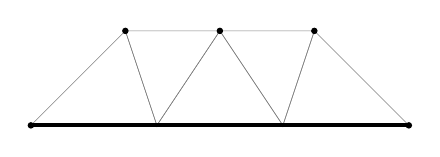
\begin{tikzpicture}[scale=1.200000]
  \draw[gray,very thin] (0.666667,0.000000) -- (0.000000,1.000000) -- (-0.666667,0.000000) -- (0.666667,0.000000) ;
  \draw[gray,very thin] (0.666667,0.000000) -- (2.000000,0.000000) -- (1.000000,1.000000) -- (0.666667,0.000000) ;
  \draw[gray,very thin] (-2.000000,0.000000) -- (-0.666667,0.000000) -- (-1.000000,1.000000) -- (-2.000000,0.000000) ;
  \draw[gray,very thin] (-0.666667,0.000000) -- (0.000000,1.000000) -- (-1.000000,1.000000) -- (-0.666667,0.000000) ;
  \draw[gray,very thin] (0.666667,0.000000) -- (1.000000,1.000000) -- (0.000000,1.000000) -- (0.666667,0.000000) ;
  \filldraw (2.000000,0.000000) circle (0.800000pt);
  \filldraw (1.000000,1.000000) circle (0.800000pt);
  \filldraw (-1.000000,1.000000) circle (0.800000pt);
  \filldraw (-2.000000,0.000000) circle (0.800000pt);
  \filldraw (0.000000,1.000000) circle (0.800000pt);
  \filldraw (-0.666667,0.000000) circle (0.300000pt);
  \filldraw (0.666667,0.000000) circle (0.300000pt);
  \draw[line width=1.500000pt] (-2.000000,0.000000) -- (-0.666667,0.000000);
  \draw[line width=1.500000pt] (-0.666667,0.000000) -- (0.666667,0.000000);
  \draw[line width=1.500000pt] (0.666667,0.000000) -- (2.000000,0.000000);
\end{tikzpicture}
